\section{The Standard Model} \label{sec:theory:standardmodel}

At the turn of the 20th century our understaning of the constituent matter of
the universe was limited to what we could see with microscopes and imply from
the observations of light and elctricity, giving us evidence for both the photon
and the electron.  In the first half of the century we discovered the field of
subatomic physics with Rutherfords 1911 gold foil scattering experiment, and
Dirac successfully demonstrated the quantization of the electromagnetic field,
the first step towards a fully Gauge Invariant Quantum Field Theory.  In the
second half we literally delved deeper, discovering that the nucleus contained
structure and extended our theories to include the the complex mechanics of
quarks and gluons.  With the discovery of the Higgs in 2013 the Standard Model
has become an irrefutable framework as can be seen in the high level of
agreement betwee theory experiment in \Cref{fig:xsection_measurements}.

\begin{figure}[!htbp]
  \begin{center}
    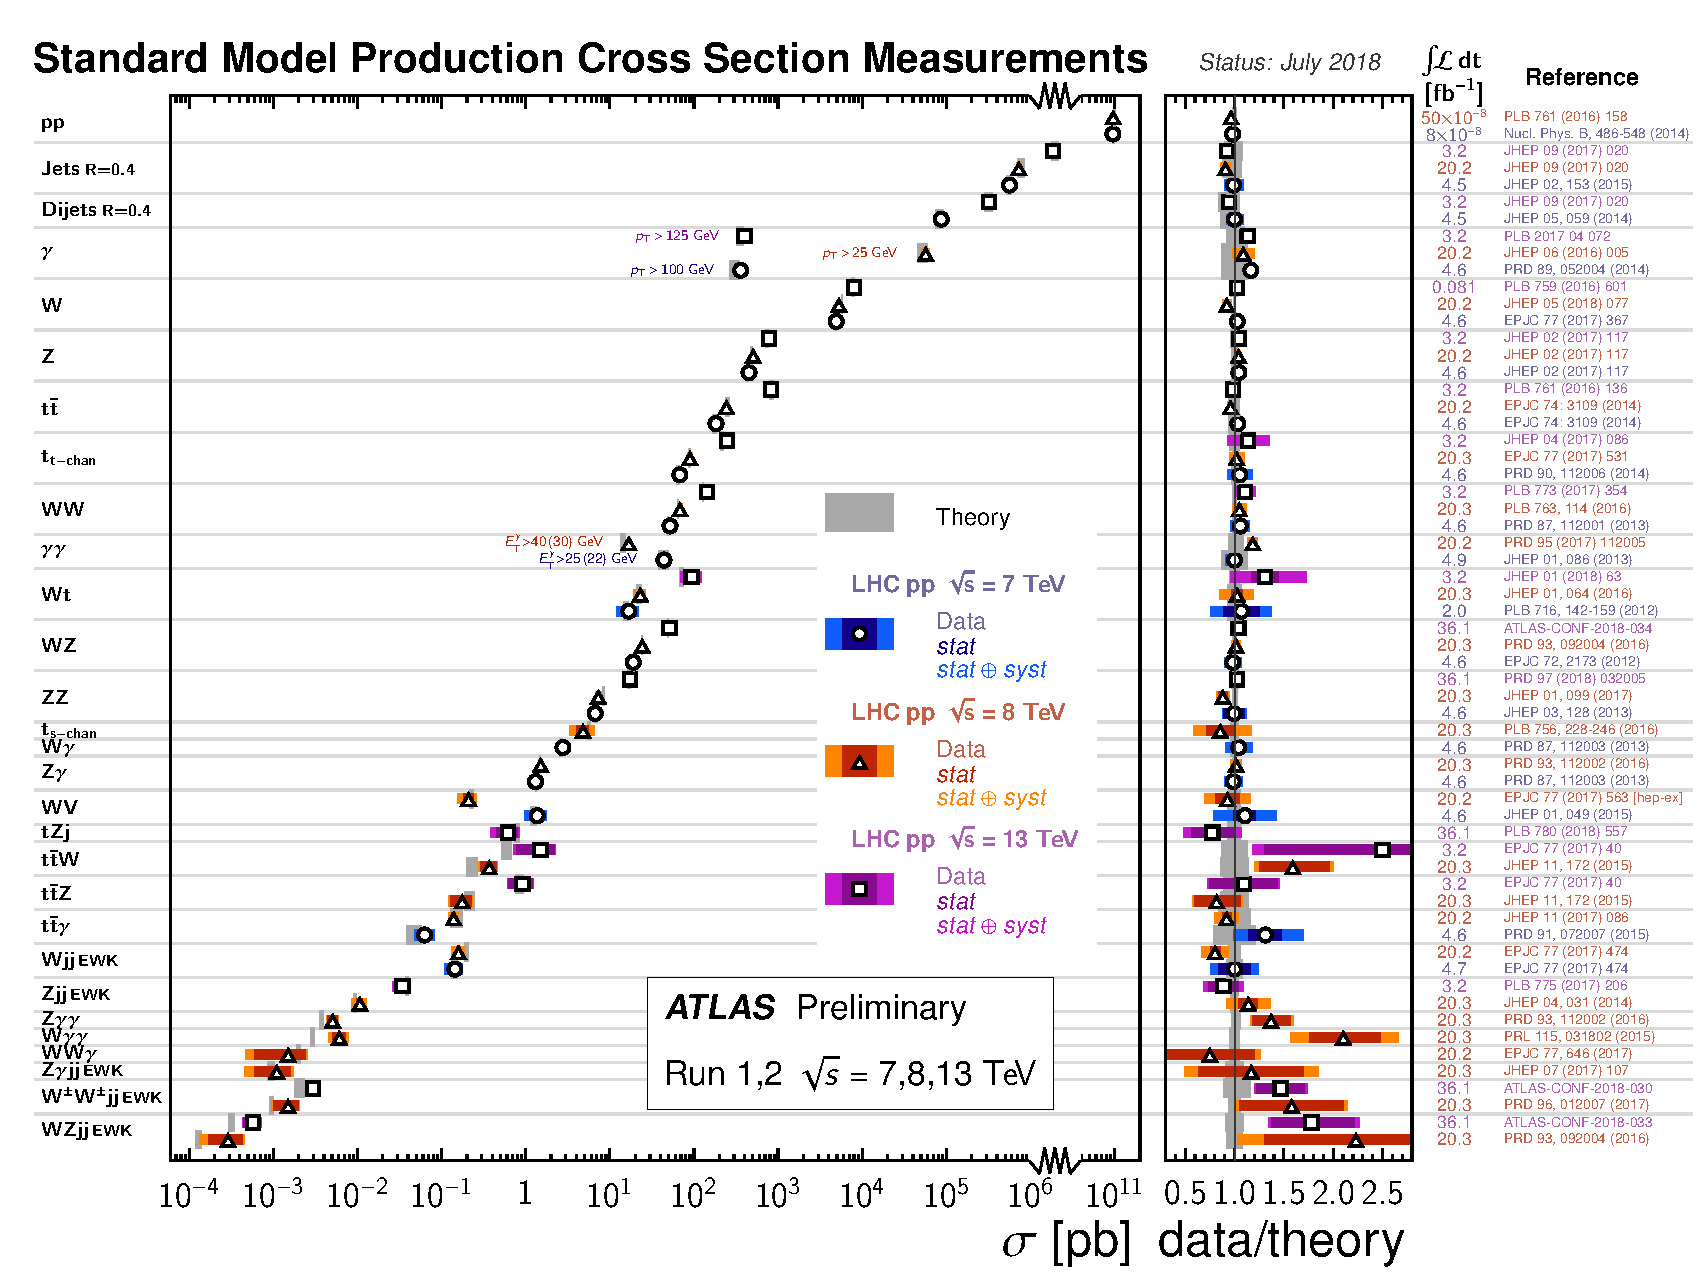
\includegraphics[width=0.8\linewidth]{figures/theory/xsection_measurements.pdf}
    \caption{ Summary of several Standard Model total and fiducial production cross section measurements, corrected for leptonic branching fractions, compared to the corresponding theoretical expectations. All theoretical expectations were calculated at NLO or higher. The dark-color error bar represents the statistical uncertainty. The lighter-color error bar represents the full uncertainty, including systematics and luminosity uncertainties. The data/theory ratio, luminosity used and reference for each measurement are also shown. Uncertainties for the theoretical predictions are quoted from the original ATLAS papers. They were not always evaluated using the same prescriptions for PDFs and scales. The Wgamma and Zgamma theoretical cross-sections have non-perturbative corrections applied to the NNLO fixed order calculations (PRD 87, 112003 (2013)). Not all measurements are statistically significant yet.}
    \label{fig:xsection_measurements}
  \end{center}
\end{figure}

The QCD and QED theories predict two classes of particles: fermions and bosons
shown in \Cref{fig:standard_model}. These particles represent the quanta
of the quantum fields of the Standard Model and the mediators of the fundamental
forces of Nature.

\begin{figure}[!htbp]
  \begin{center}
    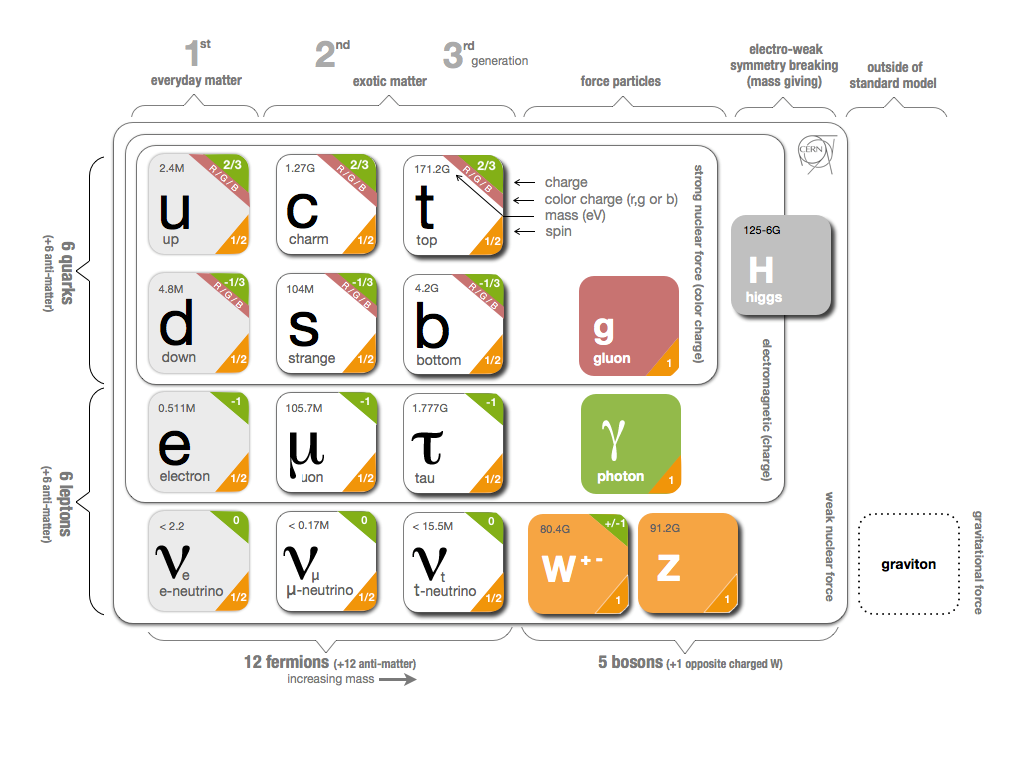
\includegraphics[width=0.8\linewidth]{figures/theory/standard_model.png}
    \caption{ Table of all observed fundamental particles of the current
Standard Model.}
    \label{fig:standard_model}
  \end{center}
\end{figure}

\subsection{Bosons} \label{sec:theory:bosons}

These spin-1 particles are known as the vector gauge bosons and are the
force carriers of the SM.  The most commonly known is the electromagnetic
force's un-charged and massless photon ($\gamma$) which interacts with all
charged particles and is often refered to as "light".  The weak nuclear force is
involved in nuclear interactions such as beta decays and is carried by 3 bosons
all of which have mass and couple to all fermions; the $W^{\pm}$ bosons, which
mediate the charged weak nuclear interaction and allow for flavor changing
currents; and the $Z$ boson which mediates the neutral weak nuclear interaction.
Finally we have 8 massless gluons which mediate the strong nuclear force and
only interact with fermions with a "color" charge such as the quarks contained
inside the nucleus. The only spin-0 boson, the Higgs Boson ($h$) is the key to
generating mass terms in the SM Lagrangian for the massive Gauge Bosons and for
fermions.  This is done through the so called Higgs Mechanism and is discussed
in more detail in \Cref{sec:theory:higgs}.

\subsection{Fermions} \label{sec:theory:fermions}

These spin-1/2 particles can be further broken up into two distinct familes of
particles, the leptons and the quarks, both of which contain three "generations"
each with an "up" and "down" type particle.  The leptons "up" type members are
the electrically charged electron ($e$), muon ($\mu$) and tau ($\tau$) while the
"down" type are their electrically neutral counterparts $\nu_e$, $\nu_\mu$,
$\nu_\tau$. The quarks "up" type members are the up ($u$), charm ($c$), and top
($t$) each with a $+2/3$ elementary charge, while the "down" type members are
the down ($d$), strange ($s$), and bottom ($b$) all of which have a $-1/3$
elementary charge.  Each quark carrys a "color" charge thus allowing them to
participate in strong force interactions.  Due to the observed color confinement
of the strong force these quarks are only observed in colorless bound states
known as "mesons" (1 quark and 1 anti-quark) and "baryons" (an odd number of
quarks and anti-quarks).  All of the above fermions have an anti-particle
partner which has the opposite electrical charge but is otherwise identical.
